\documentclass[12pt]{article}
\usepackage{graphicx}

\begin{document}
	
\noindent {\LARGE\textsc{Física Computacional-I}}\par
\bigskip
\noindent {\large\textsc{Tarea 1}}\par
\noindent\hrulefill

\section{Teoría}

\subsection{Coeficientes Binomiales}

 Los Coeficientes Binomiales, que generalmente se representan como${n\choose k}$ son enteros que corresponden al número de formas en que se puede extraer subconjuntos a partir de un conjunto. Se pueden calcular con la siguiente expresión

\begin{equation}
{n\choose k} = {n!\over k!(n-k)!}
  = {n\times(n-1)\times(n-2)\times\ldots\times(n-k+1)\over
     1\times2\times\ldots\times k}
\end{equation}\label{Equa1}

con $k\ge1$ y ${n\choose0}=1$ si $k=0$.

\subsection{El triángulo de Pascal o triángulo de coeficientes binomiales}

Es una representación de los coeficientes binomiales ordenados en forma de triángulo. donde los renglones corresponden a n = 0, 1, 2, 3, 4, .. Para cada n, el n-ésimo renglón está formado por los números ${n\choose k}$, con $k = 0, 1, . . . , n$, ver Figura \ref{fig:pascal}.

\begin{figure}
	\centering
	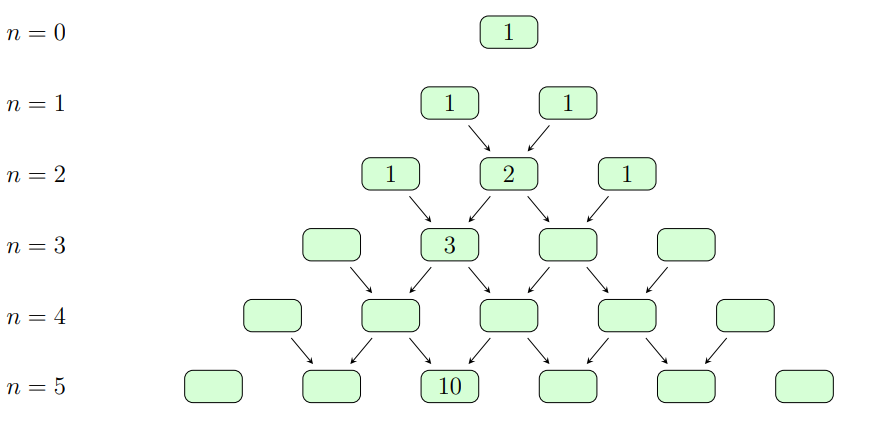
\includegraphics[width=0.8\textwidth]{Pascal.png} 
	\caption{Representación del triángulo de Pascal. Las flechas muestran cómo funciona la fórmula recursiva: cada elemento (excepto los elementos extremos en cada fila) se obtiene como la suma de dos elementos de arriba.}
	\label{fig:pascal}
\end{figure}




\section{Ejercicios}

Cree un repositorio en GitHub llamado Tarea1\_Nombre\_Apellido en su cuenta, debe de sincronizar el codigo con dicho repositorio.

Todas las funciones deben de ser creadas dentro de un módulo llamado funciones.py para que pueda ser llamado por el programa principal que se debe de llamar Tarea1.py.

\begin{enumerate}\setlength{\itemsep}{0pt}
	
\item Cree una función \texttt{Factorial(n)} que reciba un numero $n$ y entregue $n!=n\times(n-1)\times(n-2)...\times2$.

\item Construya una función \texttt{Binomial(n,k)}, que dados los enteros $n, k$ calcule y entregue los correspondientes coeficientes binomiales según la ecuación \ref{Equa1}

\item Con la ayuda de la \texttt{Binomial(n,k)} construya una función llamada \texttt{Pascal(n)} que genere un triangulo de pascal de $n$ lineas y lo guarda en un archivo con nombre Pascal-n.txt.
  
\item La probabilidad de que cuando se lanza una moneda $n$ veces resulte un número $k$ de veces cara (sello) está dada por la expresión ${n\choose k}/2^n$. Usando el módulo que ya escribió escriba una rutina dentro de Tarea1 que calcule e imprima (a) la probabilidad de que si se hace este experimento 100 veces, el resultado sean 10 veces cara, (b) la probabilidad de que caiga cara más de 30 veces.


\end{enumerate}

\subsection{Checks}

\begin{enumerate}
	\item Tanto la función \texttt{Binomial(n,k)} como \texttt{Factorial(n)} solo pueden recibir enteros y entregar enteros.
	
	
\item Su trinágulo debe tener esta forma
\begin{flushleft}
n=0~~~~~~1\\
n=1~~~~~1 1 \\
n=2~~~~1 2 1 \\
n=3~~~1 3 3 1 \\
n=4~~1 4 6 4 1\\
.\\.\\.
\end{flushleft}
\item Todas las funciones deben de estar debidamente comentadas

\item Cree un programa dentro de un archivo test.py que pruebe cada una de las funciones. Esto es utilice resultados conocidos para testear que sus funciones estén haciendo lo que deben.
	
\end{enumerate}


\end{document}